\section{Proposed solution}\label{solution}

In a typical microservices application, who is communicating is less important than what is the data being exchanged. In order to give priority to the data rather than to hosts, we will design an Information-centric network ~\cite{Ahlgren} between microservices using NDN network stack ~\cite{zhang2014named}. This new network design will facilitate various important services like load balancing, service discovery and security features to be provided as part of our new network.

\subsection{Network services}

 \begin{enumerate}
 	\item \textbf{Service discovery}
 	 \begin{enumerate}
      	\item Each HTTP endpoint will have a unique global name in an application namespace.
    		\item Every microservice inside an application namespace will have the capability to request objects of data from any other endpoint inside the same namespace.
    		\item The network will have a capability to propagate requested objects through the network to the requester.
	 \end{enumerate}
 
 \item \textbf{Load balancing}
   \begin{enumerate}
    \item We will provide a capability for in-network storage ~\cite{zhang2014named} of objects which can decrease latency and improve the reliability of the application.
    \item We will provide load balancing of flows across different objects of the same version.
    \item We will give capability for different versions of the same object to coexist ~\cite{newman2015building}. 
   \end{enumerate}
   
 \item \textbf{Security features}
  \begin{enumerate}
    \item Enabling the formation of the trust domains ~\cite{dragoni2016microservices} using the concept of application namespaces[ref] to protect microservices even when an intruder gets into the system (defence in depth ~\cite{stouffer2009recommended}).
    \item We will implement service authentication as a network function for new microservices joining the network.
  \end{enumerate}
  
 \item \textbf{Improved resilience}
   \begin{enumerate}
   \item We will deliver the most recent object write from the local cache, in case of failure of an endpoint.
   \end{enumerate} 
 \end{enumerate}
 
 In order to achieve above-said goals, we describe the architecture of the new network model in next section.
 
\subsection{Implementation}
\subsubsection{Overview of design }

Each microservice will have a client library which will help connect to the NDN network. Each physical node will have a virtual NDN router capable of routing NDN packets through the network (see figure  ~\ref{fig:networkmodel}) . This NDN router will be hosted on the top of DTCP as application layer protocol[ref], this will allow us to concentrate on microservices specific functionality as replacing stack is out of the scope of this project but is possible  ~\cite{zhang2014named}. 

\subsubsection{Naming schema}

In our naming scheme, each HTTP endpoint is addressable. Every HTTP endpoint will have a globally unique name. 

\begin{center} \url{ httpendpoint/instance_count/httpend_version  } \end{center}
\begin{center} Example end point \end{center}


This naming schema is simple enough but serves to achieve required features
\begin{enumerate}
\item By using only unique HTTP endpoint name and removing reference to a microservice name, we can decouple endpoints from hosting microservices. This will help to decrease downtime and unnecessary changes when endpoints are moved between services.
\item  Having an instance count can help identify and load balance among different instances of same HTTP endpoint.
\item httpendversion helps in maintaining two versions of same end point available at the same time. this can felicitate rolling updates.  
\end{enumerate}


\subsubsection{Initial handshake}

Newly created microservice will broadcast in its own local container bridge ~\cite{DockerNet} for local NDN router IP address. Once it receives IP address it will use Named Data Link State Routing Protocol to advertise all its objects to the local router. an NDN router will only advertise longest common name for all other routers. In this way, we can have few updates while maintaining load balance between distributed endpoints.

\begin{figure}
   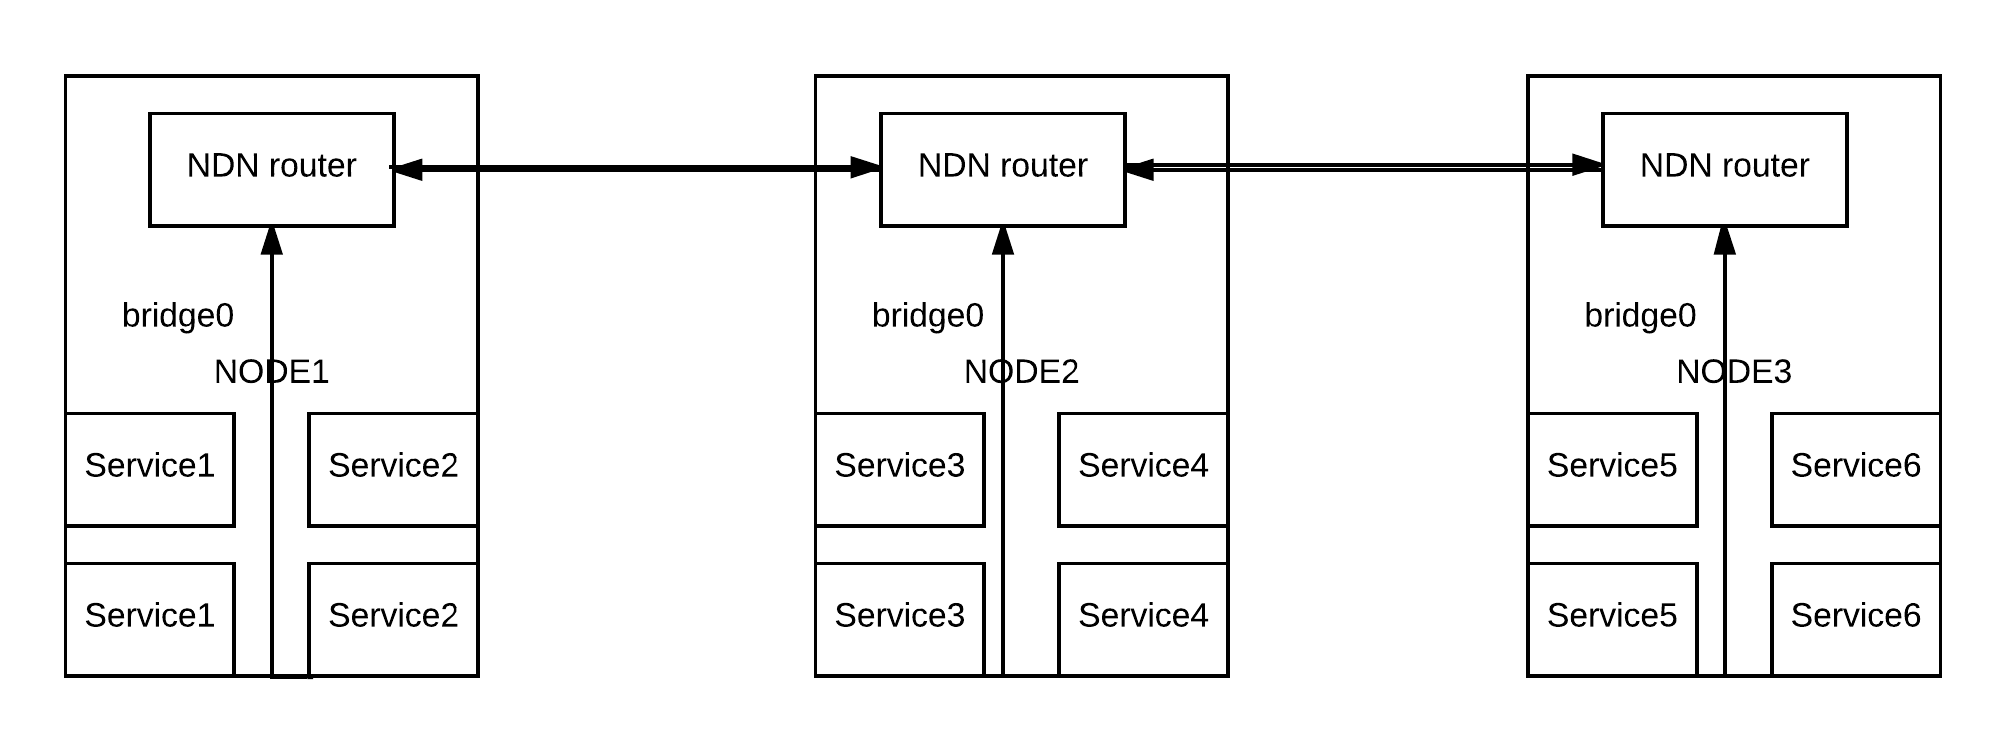
\includegraphics[height=3cm, width=8cm]{figs/structural_diagram}
   \caption{Architecture of proposed network.}
   \label{fig:networkmodel}
\end{figure}

We will implement a layer on the top of the virtual router to facilitate the initial handshake of a new HTTP endpoint and token authorization for admission of new microservice into the network.

\subsubsection{Routing}

There will be a virtual NDN node router in every physical node (see figure ~\ref{fig:networkmodel}). This router will be connected to all other containers in the same node using a bridge~\cite{DockerNet}. We will reuse NDN network stack in particularly named data network forwarding ~\cite{yuan2012scalable} and enhance its forwarding strategy to facilitate load balancing between different HTTP endpoint instances and also for different versions of HTTP endpoints to co-exist.

We will use NLSR - Named Data Link State Routing Protocol ~\cite{hoque2013nlsr} to transfer new HTTP endpoint information among router overlay network. we will only transfer routes longest matching subaddress.

\subsubsection{In-network storage}

We will implement a content cache ~\cite{zhang2014named} using memory cache in the router to facilitate in-network storage(see figure ~\ref{fig:process2}). This cache will also return most updated value of the HTTP endpoint in case of network failure.

\subsubsection{Security features}

We will use the signature section of NDN data packet ~\cite{zhang2014named} to sign with the public key supplied in the interest packet of the client. Upon receiving the requested object, the client can authenticate using the signature sent by the sender.
